Air pollution is the leading environmental health risk in many areas around the world affecting both the human population and ecology.
The effects of air pollution to the general population range from chronic to less severe health impacts, and reduced growth rates of vegetation due to air pollution results in economic losses running into billions of euros per year \citep{AQEU:2015}.
Moreover, air pollution has been labelled as carcinogenic by the International Agency for Research on Cancer \citep{IARC:2013}.
Due to these impacts, many governed areas introduced legislation designed to reduce concentrations of many air pollutants.

Tropospheric ozone (\ce{O3}) and particulate matter (PM) are the most problematic air pollutants over Europe with up to $98$ and $93$~\% of Europe's urban population exposed to concentrations of ozone and PM above the WHO guidelines \citep{AQEU:2015}.
Furthermore, in 2011 the EU ozone target value for human health (the EU does not currently have a  limit value for ozone) was exceeded in $65$~\% of the EU member states and Europe's ozone target value for vegetation was exceeded in $27$~\% of the EU-28 agricultural areas \citep{AQEU:2013}.

Reducing atmospheric concentrations of tropospheric ozone is a complex problem as ozone is not directly emitted into the troposphere.
Tropospheric ozone is produced from the reactions of nitrogen oxides \mbox{(\ce{NO_x}~$\equiv$~NO + \ce{NO2})} and volatile organic compounds (VOCs) in the presence of sunlight \citep{Atkinson:2000}.
Moreover, the photochemical nature of ozone production leads to a strong influence of meteorological variables, such as temperature and wind speed, on ozone production \citep{Jacob:2009}.

Air quality (AQ) models are an important tool for understanding ozone pollution and for predicting future air quality.
There are many AQ models available for investigating ozone pollution with different scales and dimensions depending on the scope of the modelling experiment.
Accurately representing the complexity of ozone production, such as emissions, atmospheric chemistry, meteorology and atmospheric transport, in a computationally efficient model is an ongoing challenge for the modelling community \citep{Russell:2000}.

Model intercomparison projects (MIPs) compare the outputs from different models, typically showing differences in tropospheric ozone due to differing representations of key processes.
For example, the ACCMIP (Atmospheric Chemistry and Climate Model Intercomparison Project) showed different magnitudes of future ozone burden in the same region \citep{Young:2013}.
The CCMI (Chemistry Climate Model Initiative) aims to investigate differences in the representation of chemistry, emissions and transport processes between models to understand the differences between predictions from global models \citep{Eyring:2013}.

Detailed process studies are key to understanding differences between model representations which could lead to differences in simulated ozone levels.
This thesis determines the effects of different representations of VOC degradation chemistry, VOC emissions and the effects of temperature on ozone production.
This assessment should be beneficial to the wider modelling community in understanding potential differences between model outputs and improving the current suite of models.

\section{Ozone} \label{s:ozone}
%atmospheric O3 with budget, lifetime, stratospheric & tropospheric ozone
Ozone is a atmospheric gas found in the stratosphere and troposphere, however its atmospheric effects are very different in these regions.
About 90~\% of the atmospheric ozone is present in the stratosphere with a peak mixing ratio of about $12$~ppm \citep{Seinfeld:2006}.
Stratospheric ozone absorbs the sun's ultraviolet radiation with wavelengths between $280$ and $315$~nm.
Since excess UV radiation may cause as skin cancer, cataracts and a suppressed immune system in humans, and can also damage land and aquatic ecosystems \citep{WMO:2010}, the absorption of UV radiation by stratospheric ozone is extremely important. 

In contrast, tropospheric (or surface) ozone is both a pollutant and a greenhouse gas. 
Increased levels of tropospheric ozone are harmful to humans, plants and other living systems. 
High ozone exposure may lead to pulmonary problems in humans and can decrease both crop yields and forest growth \citep{WMO:2010}. 

Globally, tropospheric ozone is mainly formed via photochemical production from the reactions of VOCs and \ce{NO_x}, described in Sect.~\ref{s:ozone_chemistry}.
Although surface ozone concentrations are also influenced by meteorology and atmospheric transport.
For example, a spring-time peak in tropospheric ozone concentrations is common in the mid-latitudes of the Northern Hemisphere originally attributed to transport of ozone from the stratosphere into the troposphere via the Stratosphere-Troposphere Exchange (STE) \citep{Monks:2000}.
However, ozone transported via STE rarely influences surface ozone levels \citep{Lelieveld:2000} and the spring maximum is due to the photochemical reactions occuring in the Northern Hemisphere spring after the buildup of reservoir species over winter \citep{Penkett:1986}.
These reservoir species are oxidised at a faster rate due to the increase in temperature, moisture and sunlight in spring.

Understanding the intracacies of surface ozone pollution requires a combined effort from the modelling, observational and chemical kinetic communities -- called the ``three-legged stool'' approach by \citet{Abbatt:2014}.
Modelling of ozone production helped in understanding the complexity of atmospheric chemistry, such as the non-linear relationship of ozone production with precursor (VOC and \ce{NO_x}) emissions.
Modelling studies attempt to reproduce observational trends of surface ozone and model predictions may inspire the set-up of new observational studies.
Chemical kinetic studies performed by laboratories give insights to missing or incorrect representations of atmospheric chemistry which may be included in updated models.

This thesis focuses on the representation of VOC degradation chemistry, VOC emissions and the ozone-temperature relationship within models and the influence on ozone production.
The state of the art knowledge of ozone production chemistry is outlined in Sect.~\ref{s:ozone_chemistry}, while sources of emissions of ozone precursors are described in Sect.~\ref{s:precursor_emissions}.
Finally, the effects of meteorology, in particular temperature, on ozone production is presented in Sect.~\ref{s:meteo_ozone}.
For the rest of this thesis, ozone shall refer to tropospheric ozone.

\section{Ozone Chemistry} \label{s:ozone_chemistry}
Ozone absorbs UV radiation producing either ground-state atomic oxygen (\ce{O(^3P)}) or excited singlet (\ce{O(^1D)}) oxygen atoms.
\begin{rxnarray}
    \ce{O3 + h\nu} & \rightarrow \ce{O2 + O(^3P)} \label{r:O3_hva} \\
    \ce{O3 + h\nu} & \rightarrow \ce{O2 + O(^1D)} \label{r:O3_hvb} 
\end{rxnarray}
Ground-state oxygen quickly reacts with oxygen to reform ozone.
\begin{rxnarray}
    \ce{O(^3P) + O2} & \xrightarrow[]{\text{\tiny{M}}} \ce{O3} \label{r:O_O2}
\end{rxnarray}
Thus there is no net loss or production of ozone through \eqref{r:O3_hva} and \eqref{r:O_O2}.
\ce{O(^1D)} may collide with \ce{N2} or \ce{O2} (represented as M in chemical reactions) stabilising to the ground-state.
\begin{rxnarray}
    \ce{O(^1D)} & \xrightarrow[]{\text{\tiny{M}}} \ce{O(^3P)} \label{r:O1D_M} 
\end{rxnarray}
This process again leads to a null cycle with ozone destruction balanced by production.
However, \ce{O(^1D)} can also react with water vapour producing two hydroxyl (OH) radicals.
\begin{rxnarray}
    \ce{O(^1D) + H2O} & \rightarrow \ce{2 OH} \label{r:O1D_H2O}
\end{rxnarray}

The OH radical is a highly reactive chemical species reacting with almost all trace chemical species in the troposphere but not relatively inert species such as \ce{N2} or \ce{O2}.
OH is primarily produced via \eqref{r:O1D_H2O} and is also catalytically produced during the degradation of VOCs.
These sources of OH together lead to a relatively high daytime concentration of OH of the order of  $10^6$~molecules~cm$^{-3}$.
\citep{Seinfeld:2006, Monks:2005}

The initial oxidation of VOCs by OH sets off a reaction chain which may lead to net production or loss of ozone depending on the atmospheric conditions.
For example, when carbon monoxide (CO) reacts with OH in the presence of oxygen, carbon dioxide and the hydroperoxy (\ce{HO2}) radical are formed.
In polluted areas with high-\ce{NO_x} concentrations, \ce{HO2} readily reacts with nitrogen oxide (NO) which regenerates OH and produces nitrogen dioxide (\ce{NO2}).
\begin{rxnarray}
    \ce{CO + OH} & \xrightarrow[]{\ce{O2}} \ce{HO2 + CO2} \label{r:CO_OH} \\
    \ce{HO2 + NO} & \rightarrow \ce{OH + NO2} \label{r:HO2_NO}
\end{rxnarray}
Photolysis of \ce{NO2} produces ground-state atomic oxygen producing ozone via \eqref{r:O_O2}.  
\begin{rxnarray}
    \ce{NO2 + h\nu} & \rightarrow \ce{NO + O(^3P)} \label{r:NO2_hv} 
\end{rxnarray}
OH may also react with NO to produce nitrous oxide (HONO), which rapidly photolyses to return OH and NO.
\begin{rxnarray}
    \ce{OH + NO} & \rightarrow \ce{HONO} \label{r:OH_NO} \\
    \ce{HONO + h\nu} & \rightarrow \ce{OH + NO} \label{r:HONO_hv}
\end{rxnarray}
However, termination of OH and \ce{NO2} regeneration occurs when OH reacts with \ce{NO2} as nitric acid (\ce{HNO3}) is formed and \ce{HNO3} may be removed through deposition processes.
\begin{rxnarray}
    \ce{NO2 + OH} \rightarrow \ce{HNO3} \label{r:NO2_OH}
\end{rxnarray}

In the low-\ce{NO_x} conditions away from polluted areas, OH and \ce{HO2} are interconverted through reactions with ozone.
\begin{rxnarray}
    \ce{OH + O3} & \rightarrow \ce{HO2 + O2} \label{r:OH_O3} \\
    \ce{HO2 + O3} & \rightarrow \ce{OH + 2 O2} \label{r:HO2_O3}
\end{rxnarray}
OH and \ce{HO2} may also react in a termination reaction producing water vapour and oxygen.
\begin{rxnarray}
    \ce{HO2 + OH} \rightarrow \ce{H2O + O2} \label{r:HO2_OH}
\end{rxnarray}
Other termination reactions involve combination reactions of \ce{HO2} radicals producing hydrogen peroxide (\ce{H2O2}).
\begin{rxnarray}
    \ce{HO2 + HO2} & \rightarrow \ce{H2O2} \label{r:HO2_HO2}
\end{rxnarray}
Hydrogen peroxide may be removed through deposition \citep{Gunz:1990} but may also be a temporary sink for the odd-oxygen species OH and \ce{HO2}, represented as \ce{HO_x}.
\begin{rxnarray}
    \ce{H2O2 + h\nu} & \rightarrow \ce{2 OH} \label{r:H2O2_hv} \\
    \ce{H2O2 + OH} & \rightarrow \ce{HO2 + H2O} \label{r:H2O2_OH}
\end{rxnarray}
In summary, the secondary degradation of CO produces ozone in high-\ce{NO_x} conditions while in low-\ce{NO_x} conditions ozone is destroyed.
\citep{Seinfeld:2006, Monks:2005}

The secondary degradation of higher VOCs has similar features to that of CO.
Methane (\ce{CH4}) with a mixing ratio of about $1.7$~ppmv is the most abundant VOC in the troposphere.
The reaction of methane with OH, in the presence of \ce{O2}, produces the methyl peroxy radical (\ce{CH3O2}) -- the simplest organic peroxy radical (\ce{RO2}).
\begin{rxnarray}
    \ce{CH4 + OH} \xrightarrow[]{\ce{O2}} \ce{CH3O2 + H2O} \label{r:CH4_OH}
\end{rxnarray}
Similar to CO oxidation, the level of \ce{NO_x} conditions play a crucial role in the fate of \ce{CH3O2} and whether ozone is produced or destroyed, this is depicted graphically in Fig.~\ref{f:CH4_oxidation}.
\begin{figure}[t]
    \begin{center}
        \caption[Methane degradation pathways]{Methane degradation pathways in low-\ce{NO_x} and high-\ce{NO_x} conditions. Taken from \citet{Monks:2005}.}
        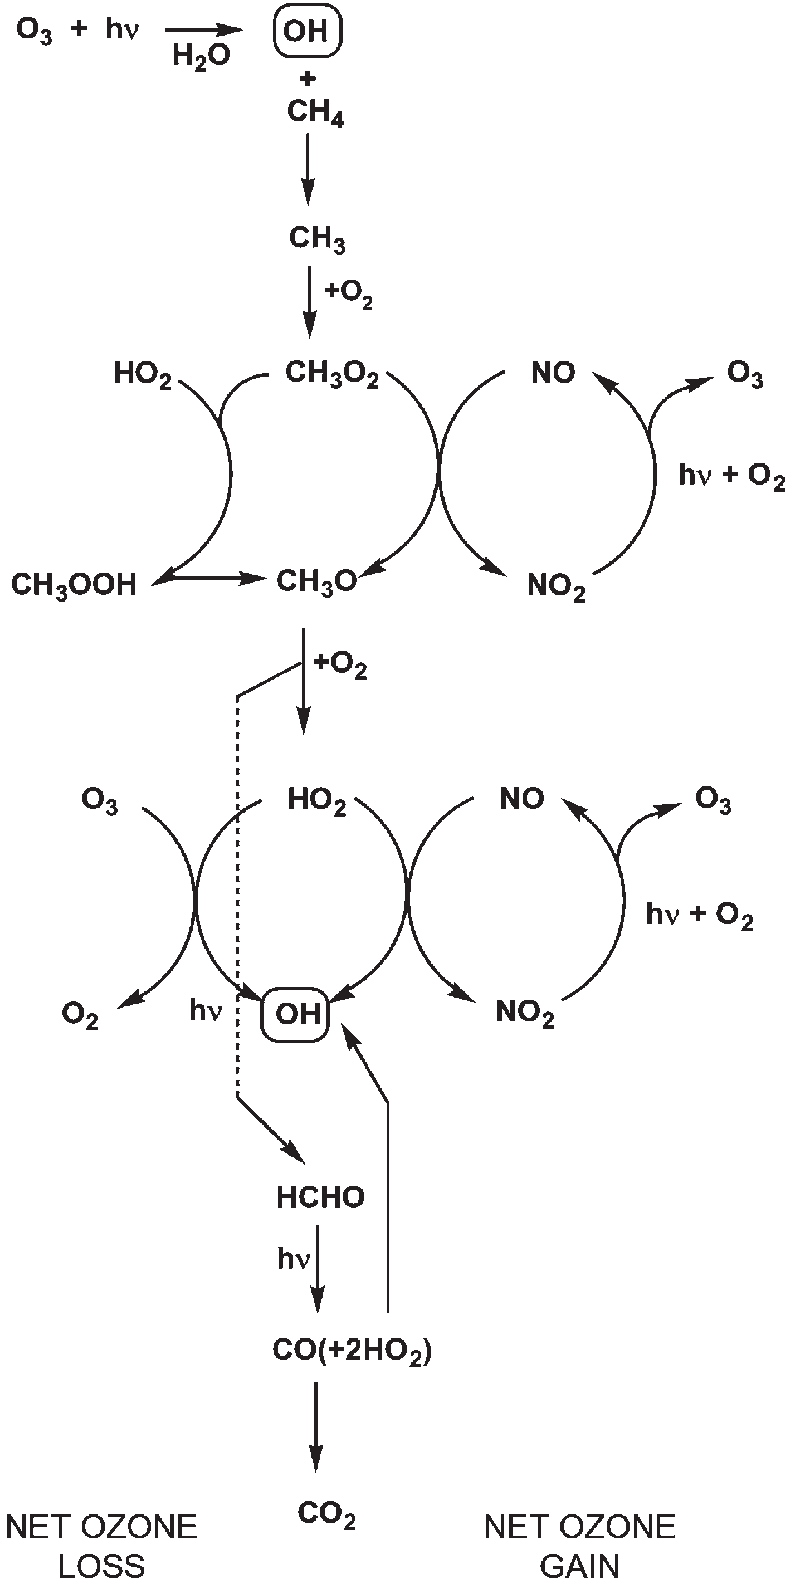
\includegraphics[scale = 0.45]{CH4_degradation}
        \label{f:CH4_oxidation}
    \end{center}
\end{figure}

The general types of secondary degradation products formed during the degradation of methane can be extended to more complex non-methane VOCs (NMVOCs).
The initial oxidation of an NMVOC may not only occur by reaction with OH.
Unsaturated VOCs, such as alkenes, may also react with ozone while photolysis is a primary degradation pathways for carbonyl species.
While during the night-time, reaction with the nitrate (\ce{NO3}) radical is typically more important than OH-oxidation due to the relatively higher concentrations of \ce{NO3} during the night-time.

\begin{rxnarray}
    \ce{VOC + OH / NO3 / O3 / h\nu} & \xrightarrow[]{\ce{O2}} \ce{RO2} \label{r:VOC_init} 
\end{rxnarray} 
\begin{figure}[t]
    \begin{center}
        \caption[Schematic of general secondary degradation of VOCs]{Schematic diagram outlining general pathways of the secondary degradation of an emitted VOC.}
        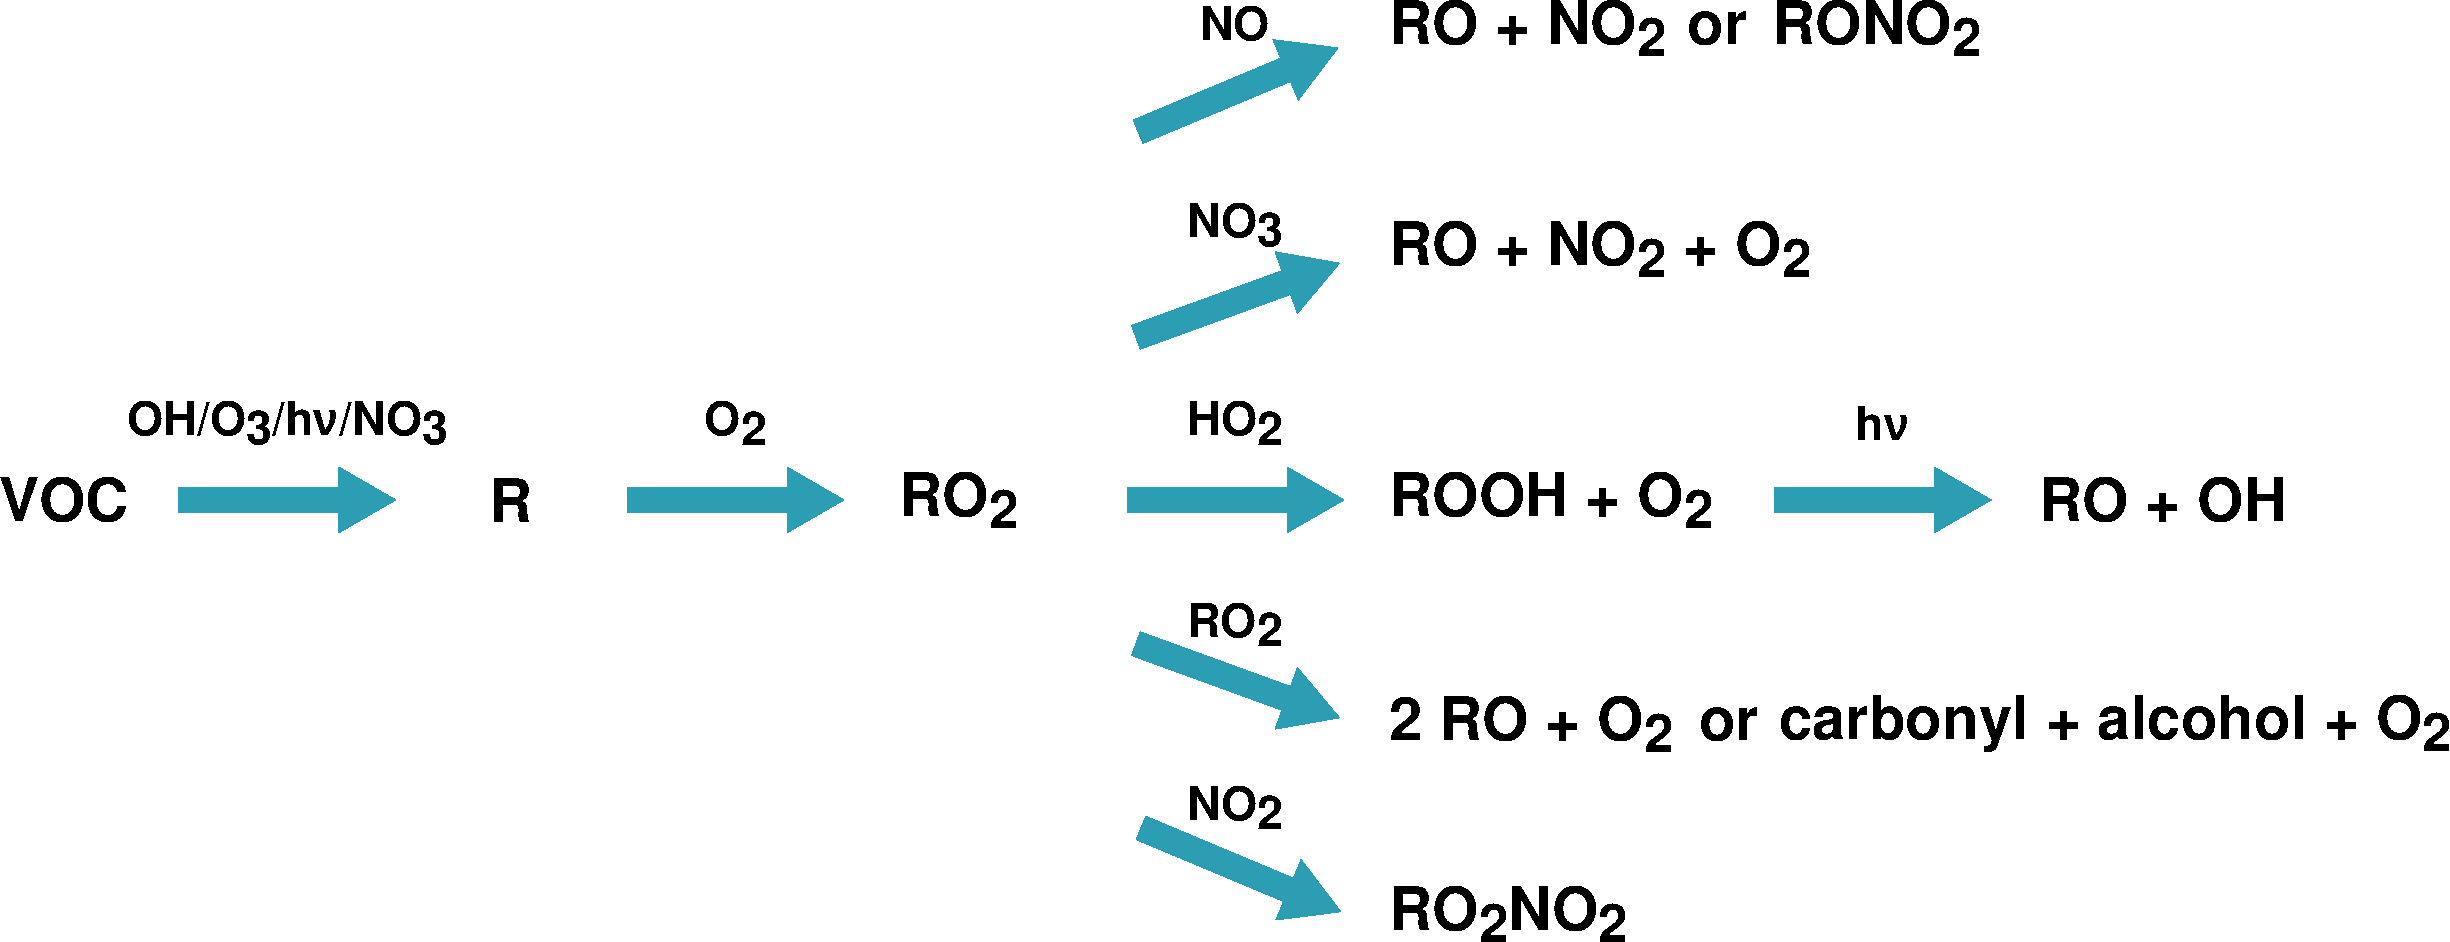
\includegraphics[width = \textwidth]{VOC_degradation}
        \label{f:VOC_reaction}
    \end{center}
\end{figure}

Figure~\ref{f:VOC_reaction} represents a general and simplified reaction scheme for VOCs in the troposphere. 
The initial oxidation of an NMVOC leads to the formation of \ce{RO2} radicals.  
Similar to CO and \ce{CH4} degradation, the fate of the peroxy radicals determines whether net loss or production of ozone occurs.
\begin{rxnarray}
    \ce{RO2 + NO} & \xrightarrow[]{\text{M}} \ce{RONO2} \label{r:RO2_NOa} \\
    \ce{RO2 + NO} & \rightarrow \ce{RO + NO2} \label{r:RO2_NOb} \\
    \ce{RO2 + NO2} & \xrightleftharpoons[]{\text{M}} \ce{RO2NO2} \label{r:RO2_NO2} \\
    \ce{RO2 + NO3} & \rightarrow \ce{RO + NO2 + O2} \label{r:RO2_NO3} \\
    \ce{RO2 + HO2} & \rightarrow \ce{ROOH + O2} \label{r:RO2_HO2} \\
    \ce{RO2 + RO2} & \rightarrow \ce{2RO + O2} \label{r:RO2_RO2a} \\
    \ce{RO2 + RO2} & \rightarrow \ce{RCH(OH)R + RC(O)R + O2} \label{r:RO2_RO2b}
\end{rxnarray}
All reactions pathways of \ce{RO2} that produce \ce{NO2} while simultaneously recycling radicals can result in \ce{O3} formation due to \eqref{r:NO2_hv} and \eqref{r:O_O2}. 
Reaction with the \ce{HO2} radical forms a hydroperoxide (ROOH) which may either be removed from the system or photolyse to produce an alkoxy (RO) radical and OH.
The carbonyl and alcohol products resulting from reaction with other \ce{RO2} radicals will follow a similar sequence of reactions and hence can also produce further \ce{O3}. 
Thus the subsequent reactions of secondary degradation products, also called the secondary chemistry, of a VOC may lead to further production of ozone.

Reaction of \ce{RO2} with \ce{NO2} forms peroxynitrates (\ce{RO2NO2}) which are a temporary reservoir for \ce{RO2} and \ce{NO_x}.
The thermal decomposition rate of \ce{RO2NO2} is highly temperature dependent.
Hence, at lower temperatures \ce{RO2NO2} may build up and be transported away from the region of formation and re-release \ce{RO2} and \ce{NO2} downwind fuelling ozone production away from large sources of \ce{NO_x}.
This is one example of the dependence of ozone production on meteorological variables, a broader overview is given in Sect.~\ref{s:meteo_ozone}.

Another important reaction involving ozone in polluted regions is that of NO with \ce{O3}.
\begin{rxnarray}
    \ce{NO + O3} & \rightarrow \ce{NO2 + O2} \label{r:NO_O3}
\end{rxnarray}
Together with \eqref{r:NO2_hv} and \eqref{r:O_O2}, this is a very important null cycle of ozone production and destruction.
In polluted areas with high NO emissions or in the night-time when no photochemistry occurs, the concentration of ozone is limited by the rates of \eqref{r:NO_O3} and \eqref{r:NO2_hv}.

\subsection[VOC and NOx Chemistry]{VOC and \ce{NO_x} Chemistry} \label{ss:VOC_NOx}
\begin{figure}
	\begin{center}
        \caption[Ozone mixing ratios as a function of \ce{NO_x} and VOC]{Ozone isopleth plots for various initial mixing ratios of \ce{NO_x} and a VOCs. Taken from \citet{Jenkin:2000}.}
        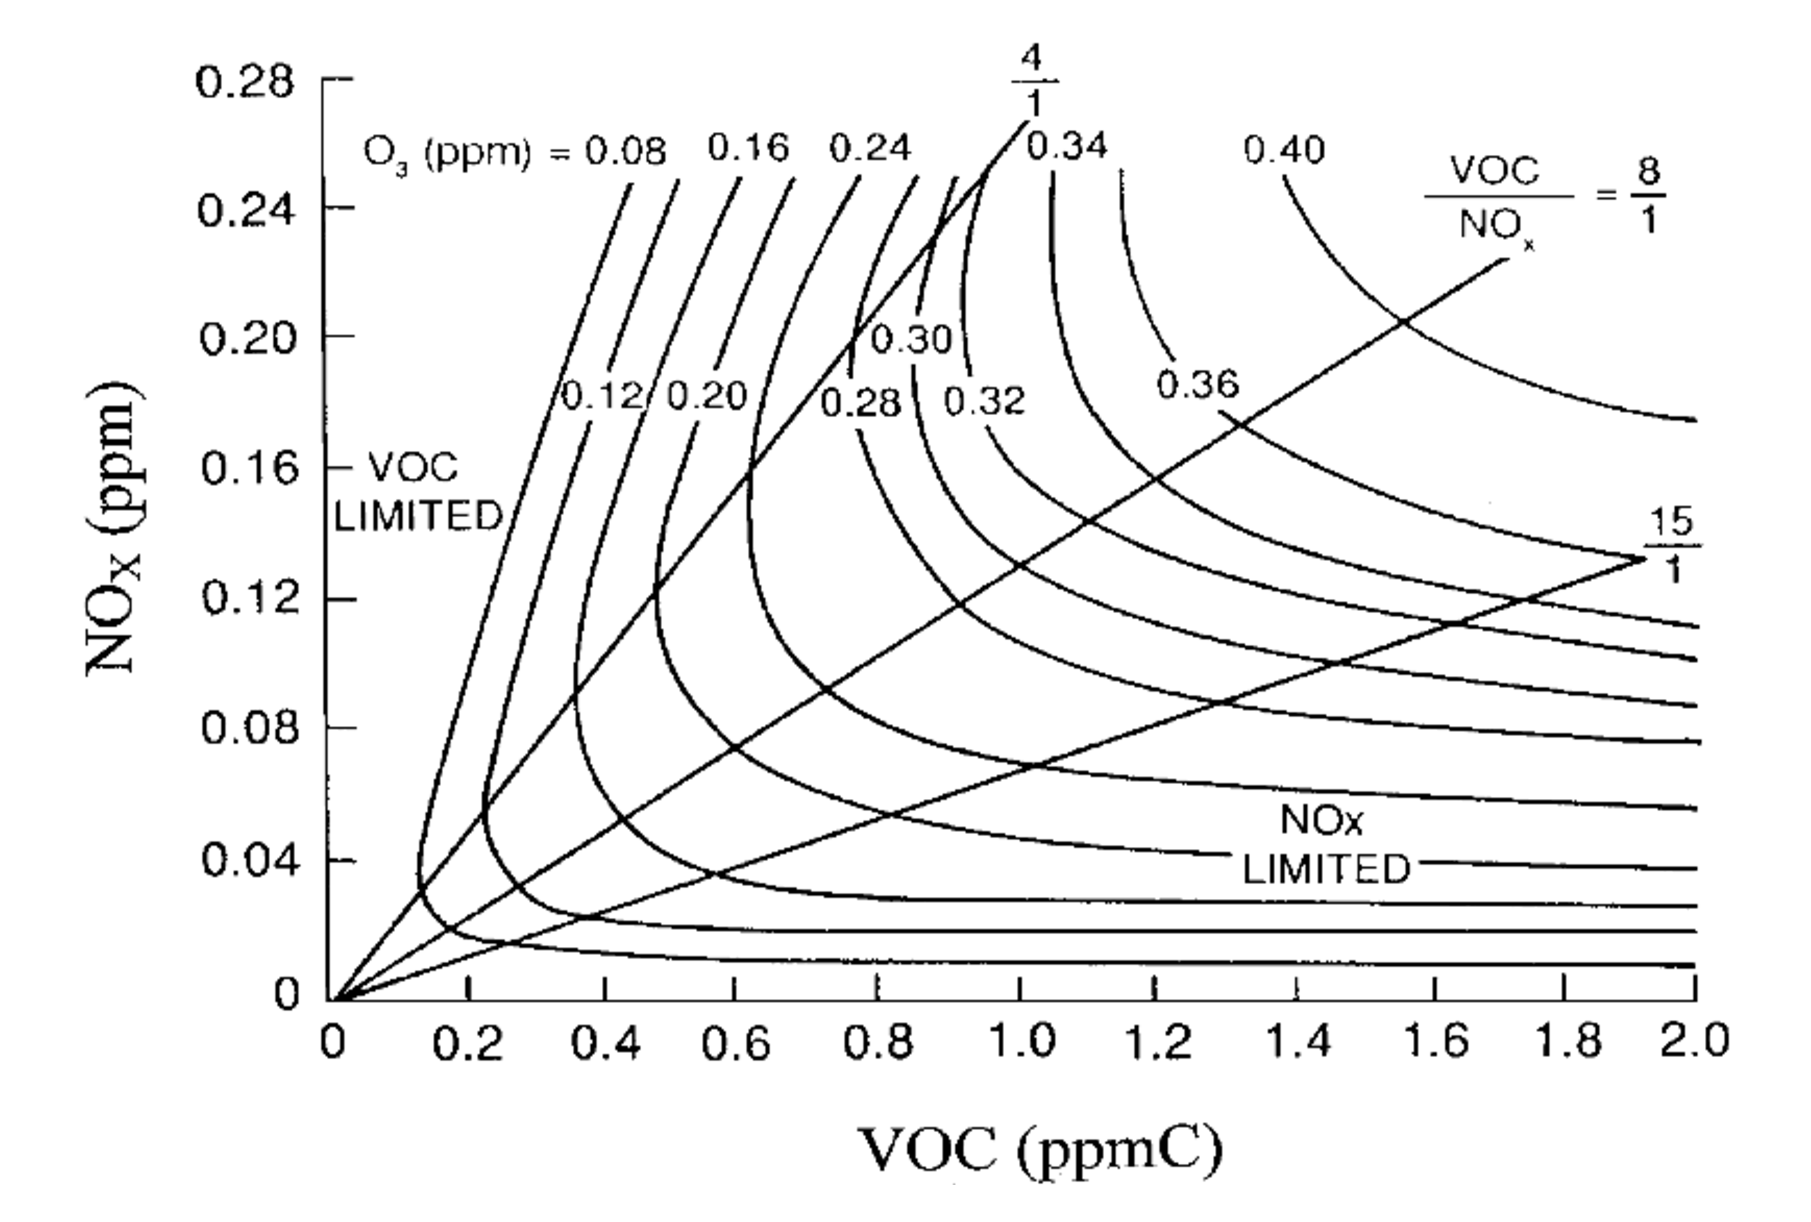
\includegraphics[width = 0.9\textwidth]{O3_isopleth}
		\label{f:O3_isopleth}
	\end{center}
\end{figure}
%balance of NOx & NMVOC for O3 production
The fate of peroxy radicals produced during VOC degradation depends on the ratio of the concentrations of radicals and \ce{NO_x} \citep{Kleinman:1991, Kleinman:1994}.
In regions with low-\ce{NO_x} concentrations, \ce{RO2} are more likely to react with other radicals rather than convert NO to \ce{NO2}, leading to ozone production.
The most common reactions are bimolecular destruction \eqref{r:HO2_OH}, which removes radicals, or combination of radicals \eqref{r:RO2_HO2} into reservoir species that may re-release radicals.
This is \emph{\ce{NO_x}-sensitive} chemistry.

On the other hand, when \ce{RO2} reacts with \ce{NO2} in regions with high levels of \ce{NO_x}, the production of \ce{HNO3} increases \eqref{r:NO2_OH}.
Nitric acid is a sink for both OH and \ce{NO_x} removing OH which would otherwise react with emitted VOC to fuel further radical production.
This is \emph{VOC-sensitive} or \emph{\ce{NO_x}-saturated} chemistry.

The different chemistry in low-\ce{NO_x} and high-\ce{NO_x} areas indicates that ozone production is a non-linear process.
Figure~\ref{f:O3_isopleth}, from \citet{Jenkin:2000}, depicts the non-linear relationship between \ce{O3} mixing ratios as a function of VOC and \ce{NO_x} mixing ratios.  
This relationship can be divided into distinct regimes of ozone production: \emph{\ce{NO_x}-sensitive} (or \emph{\ce{NO_x}-limited}), \emph{\ce{NO_x}-saturated} (or \emph{VOC-sensitive}) and \emph{VOC-and-\ce{NO_x}-sensitive} regimes. 

In the \ce{NO_x}-sensitive regime, increasing \ce{NO_x} increases the number of NO to \ce{NO2} reactions by peroxy radicals leading to ozone production.
However, increasing VOC levels has little effect on \ce{O3} production due to increased radical-radical reactions.

The \ce{NO_x}-saturated regime corresponds to high \ce{NO_x} concentrations where radicals will tend to react with \ce{NO_x}. 
Increasing levels of VOC increase the liklihood of \ce{RO2} converting NO to \ce{NO2} while increasing \ce{NO_x} levels will not increase \ce{O3} production.

The VOC-and-\ce{NO_x}-sensitive regime is characterised by \ce{O3} production being sensitive to both VOC and \ce{NO_x} levels. 
Morever, it is in this atmospheric regime that the maximum amount of ozone is produced and corresponds to the contour ridges in Fig.~\ref{f:O3_isopleth}.
\citet{Kleinman:1994} showed that this non-linear relationship can be thought of as a titration process between radicals and \ce{NO_x} with the VOC-and-\ce{NO_x}-sensitive regime being the turning point.

The non-linear nature of ozone production is one of the challenges in controlling ozone levels.
The difficulty is exacerbated by the fact that regions can alternate between these regimes depending on the meteorological conditions.
Moreover, fresh emissions tend to occur in \ce{NO_x}-saturated areas before being transported to VOC-and-\ce{NO_x}-sensitive and \ce{NO_x}-sensitive regions.

\subsection{Representing Atmospheric Chemistry in Models} \label{ss:chemistry_models}
Representing the complex chemistry for each emitted VOC in a chemical transport model (CTM) is unrealistic.
Even if all the secondary degradation pathways and products were known for every VOC, a CTM would not be able to efficiently numerically solve the resulting differential equations.
Hence, CTMs use descriptions of atmospheric chemistry that lead to more computationally efficient models \citep{Stockwell:2012}.

The representation of atmospheric chemistry in a CTM is called a chemical mechanism of which there are many choices.
The choice of chemical mechanism depends on the scope of the modelling study and typically only one chemical mechanism is used.

Chemical mechanisms are developed by simplifying and aggregating degradation products, VOCs and reactions.
Less aggressive simplification approaches may result in a chemical mechanism having thousands of species while more aggressive simplification may result in only a hundred species. 
Chemical mechanisms are verified by comparing the concentrations of field studies or controlled chamber study experiments to model simulations \citep{Stockwell:2012}.
Section~\ref{s:chemical_mechanisms} includes further details of the simplification techniques used to develop chemical mechanisms.

Chemical mechanism comparison studies, such as \citet{Kuhn:1998} and \citet{Emmerson:2009}, compare the outputs of different chemical mechanisms using the same model setup and initial conditions.
These studies show that the differences in representing atmospheric chemistry can lead to large differences in simulated ozone concentrations.
These comparisons of the concentrations of key atmospheric species, such as ozone, OH, peroxynitrates and \ce{NO_x}, indicate that the chemistry leads to differences but does not help in pointing out the root cause.

Determining where the source of differences between chemical mechanisms is a difficult task due to the interlinked chemistry of many key species.
As part of this study, the ozone production from different chemical mechanisms is compared and differences in the treatment of VOC degradation chemistry is determined aiding the future development of chemical mechanisms.
The research questions driving this comparison are presented in Sect.~\ref{s:research_questions} and the results are described in Sect.~\ref{s:chemical_mechanism_results}.

\section{Source and Sinks of Ozone Precursors} \label{s:precursor_emissions}
%temporal profile of emissions
Ozone precursors (\ce{NO_x} and VOCs) are emitted from many anthropogenic and biogenic sources.
Moreover, emissions may vary throughout the year, month or time of day.
In many regions, reduced road transport during the weekend leads to a noticible reduction in \ce{NO_x} emissions influencing ozone levels.
This is called the ``weekend-effect''.
For example, ozone production is \ce{NO_x}-saturated during weekdays in San Joaquin Valley, California but during the weekend higher ozone levels are recorded as the reduction in \ce{NO_x} levels leads to VOC-and-\ce{NO_x}-sensitive chemistry \citep{Pusede:2014}.

Anthropogenic and biogenic emissions of NMVOC also have a temporal distribution.
Similar to \ce{NO_x}, many sources of NMVOC, such as industry and solvent use, have a reduction in activity during the weekend.
Transport emissions (source of both \ce{NO_x} and NMVOC) peak during the morning and evening rush hours and emissions from solvent use has a strong diurnal cycle.
Residential combustion is highest during the winter months and lowest during the summer \citep{Gon:2011}.

% NOx sources and quantities, weekend effect
\subsection[NOx]{\ce{NO_x}}
Anthropogenic activities are the main source of \ce{NO_x} emissions into the atmosphere.
In the year 2000, almost $52$~Tg~N were emitted with 65~\% through the many forms of fossil fuel combustion \citep{Seinfeld:2006}. 
Examples of fossil fuel combustion emitting \ce{NO_x} are transportation using diesel or petrol vehicles, industrial activities and domestic heating \citep{vonSchneidemesser:2015}.

Up to $95$~\% of \ce{NO_x} emissions from combustion are emitted as NO, which is then oxidised to form \ce{NO2} through \eqref{r:NO_O3} and \eqref{r:HO2_NO}.
However, due to the increase in diesel vehicles and the implementation of diesel filters the fraction of emitted \ce{NO2} from vehicles has increased.
\citet{Grice:2009} showed that over Europe, emissions of \ce{NO2} from diesel vehicles has increased from $8.6$~\% in 2000 to $12.4$~\% in 2004.

Despite the overwhelming majority of \ce{NO_x} emissions coming from human activities, there are many important natural sources of \ce{NO_x}.
Lightning is an important source of \ce{NO_x} in the free troposphere while emissions of \ce{NO_x} from soils are important in remote regions with little anthropogenic influence.
Lightning and soils each contributed about $10$~\% to global \ce{NO_x} emissions in 2000 \citep{Seinfeld:2006}.

The deposition of nitric acid, formed via \eqref{r:NO2_OH}, is the main sink of \ce{NO_x} in the atmosphere.
Temporary reservoirs, such as peroxynitrates and HONO, may be transported away from the source region moving \ce{NO_x} away from its sources into areas devoid of large sources of \ce{NO_x}.
These sources and sinks of \ce{NO_x} are illustrated in Fig.~\ref{f:NOx_sources_sinks}.
\begin{figure}[t]
	\begin{center}
        \caption[\ce{NO_x} sources and sinks]{The sources and sinks of \ce{NO_x}, adapted from \citet{Seinfeld:2006}.}
        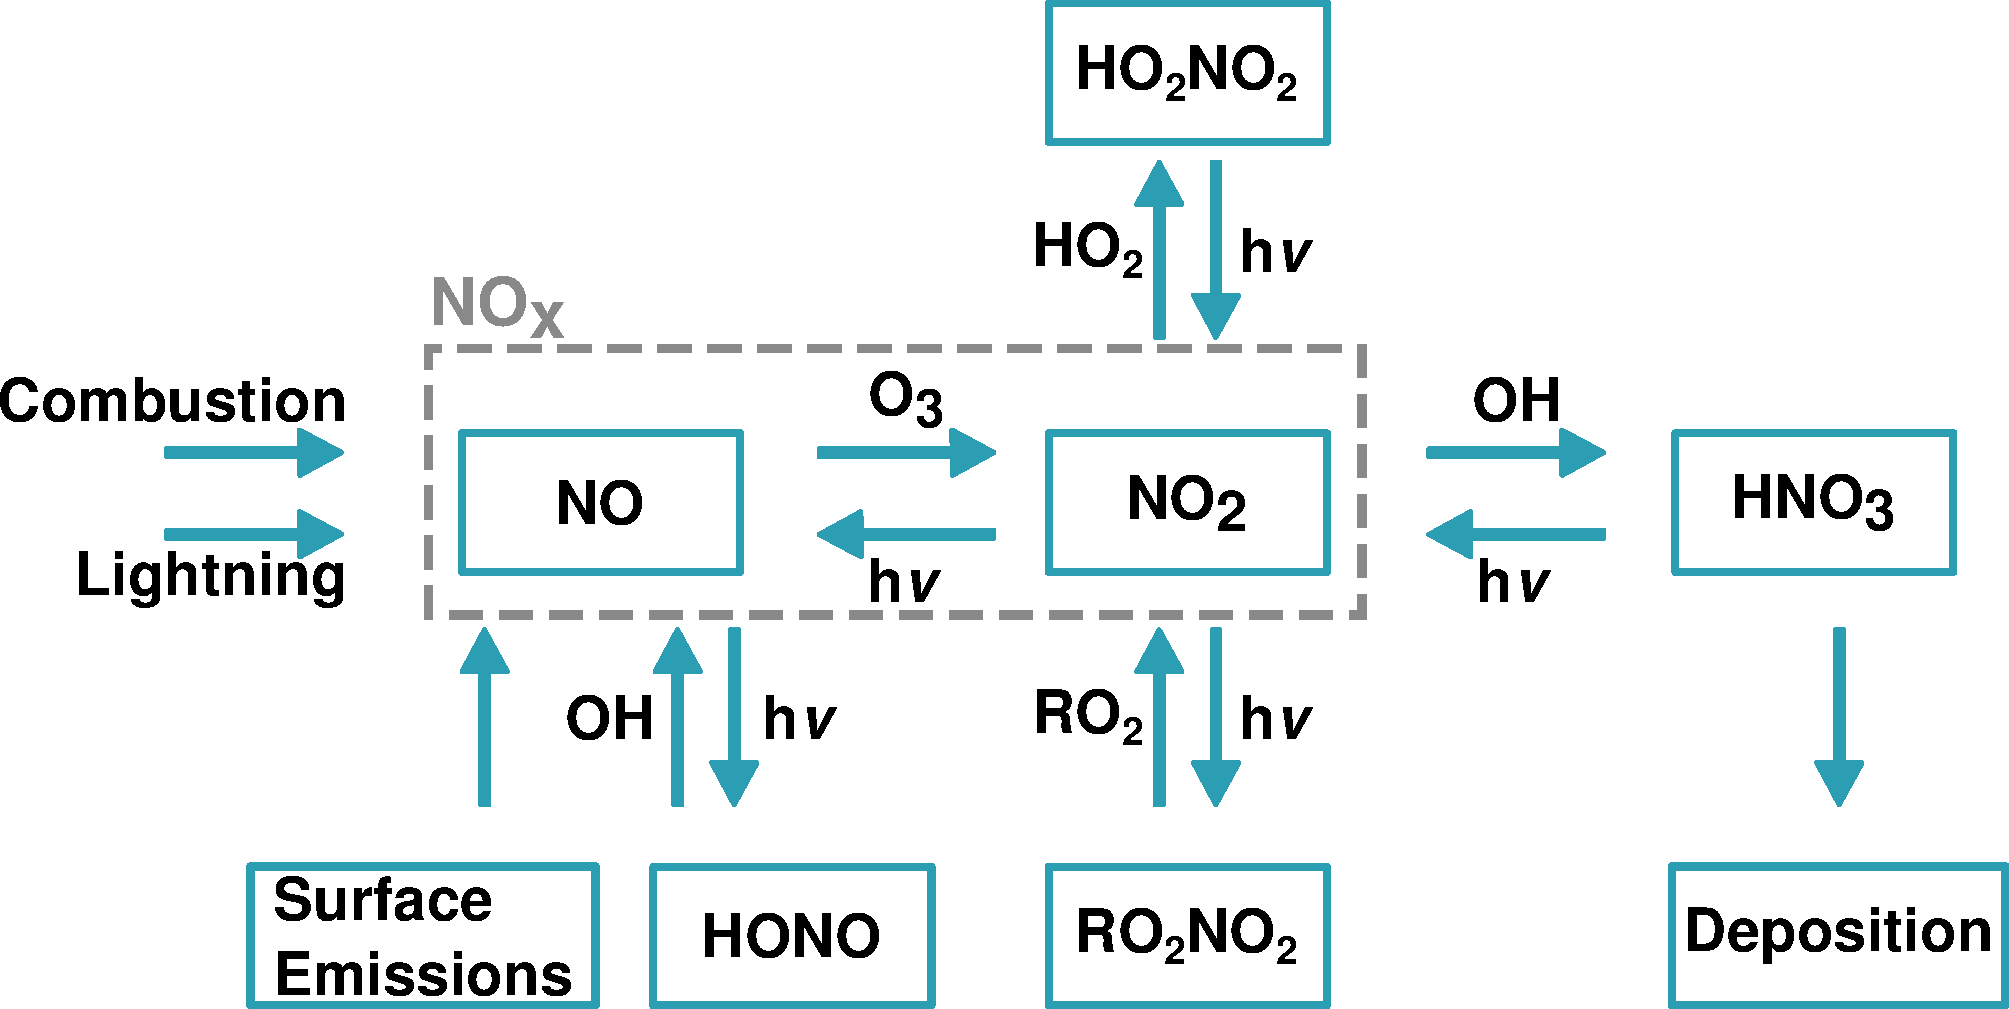
\includegraphics[width = \textwidth]{NOx_sources_sinks}
        \label{f:NOx_sources_sinks}
	\end{center}
\end{figure}

\subsection{VOCs}
The main sinks of VOCs is the oxidation chemistry tied to ozone production described in Sect.~\ref{s:ozone_chemistry}.
The degradation of a VOC yields the maximum possible amount of ozone when every peroxy radical converts NO to \ce{NO2} ans is called the \emph{ozone production potential} (OPP) of a VOC.
In reality, the OPP of a VOC is never achieved as other reactions with peroxy radicals occur however the OPP is a useful way of assessing the amount of ozone produced from emitted VOCs.

\subsubsection{Carbon Monoxide}
Carbon monoxide is emitted directly into the troposphere through combustion and industrial processes.
Another equally-important source of CO, is its chemical formation during the degradation of VOCs.
\citet{Hauglustaine:1998} estimated that $881$~Tg~yr$^{-1}$ of CO was produced globally from chemical oxidation of VOC while $1219$~Tg~yr$^{-1}$ of CO was directly emitted.

As described in Sect.~\ref{s:ozone_chemistry}, the main sink of CO is by reacting with OH \eqref{r:CO_OH}.
The OPP of CO is $1$ as the degradation sequence of CO oxidation produces only \ce{HO2}, thus a maximum of one molecule of ozone may be produced during CO degradation.

\subsubsection{Methane}
Emissions of methane are between $500$ and $600$~Tg~\ce{CH4}~yr$^{-1}$ with about $60$~\% of the emissions from anthropogenic sources.
The main anthropogenic sources of \ce{CH4} are agriculture, fossil fuels and biomass burning with agriculture contributing $60$~\% of the anthropogenically emitted methane.
Emissions from wetlands are the main natural source of methane emissions \citep{Kirschke:2013}.

Reaction with OH is the main sink of methane and this reaction is important for the concentration of OH in the troposphere.
With increased methane emissions, the concentration of OH will decrease via \eqref{r:CH4_OH} which would lead to a build of methane and other VOCs in the troposphere \citep{Holmes:2013}.

Methane (\ce{CH4}) has a lifetime of about $9$~years, significantly longer than all other VOCs.
Thus, methane influences ozone production on the global rather than the regional scale.  

The secondary degradation of methane (Fig.~\ref{f:CH4_oxidation}) produces the methylperoxy radical (\ce{CH3O2}) as well as \ce{HO2} as well as CO.
Thus methane degradation can produce a maximum five molecules of \ce{O3} per molecule of \ce{CH4} oxidised; the OPP of methane is hence $5$.

\subsubsection{NMVOCs}
%VOCs, types of VOCs and source (A vs B)
A wide variety of NMVOCs are emitted from anthropogenic activities directly into the troposphere.
Solvent use, industry, fossil fuel burning and transportation are all major activities emitting NMVOCs of varying functional groups, carbon numbers and reactivity.
Emissions of NMVOC from vegetation depends on meteorological variables (such as, temperature and radiation) and biological variables (such as, leaf age and leaf area index) \citep{Guenther:2012}.

Many NMVOCs are also hazardous to human health, especially NMVOCs associated with anthropogenic activity.
For example, benzene and formaldehyde are suspected carcinogens \citep{Laurent:2014}.
It is also worthwhile to note that the NMVOC thought to be the most hazardous to human health do not correspond to NMVOC that have a high ozone production potential.

Globally, \citet{Lamarque:2010} estimated that $130$~Tg~NMVOC were emitted from anthropogenic sources in the year 2000.
This amount is dwarfed by the total emissions from biogenic sources ($1000$~Tg~NMVOC~yr$^{-1}$) with almost eight times the amount of NMVOC emitted from anthropogenic sources \citep{Guenther:2012}.
Isoprene (\ce{C5H8}) emitted from vegetation dominates at the global scale however emissions of monoterpenes and sesquiterpenes from vegetation may also be significant.

Although isoprene is considered a biogenic VOC (BVOC), it has been measured in the urban areas of London and Paris away from natural emission sources.
Transport of isoprene is unlikely as isoprene is a highly reactive NMVOC indicating anthropogenic sources of isoprene \citep{vonSchneidemesser:2011}.
Isoprene is not the only NMVOC having both biogenic and anthropogenic sources as many small NMVOC that emitted from anthropogenic sources, such as methanol and acetaldehyde, are also emitted from vegetation \citep{Guenther:2012}.

The maximum number of molecules of \ce{O3} produced per degradation of an emitted NMVOC depends on the number of NO to \ce{NO2} conversions by the peroxy radicals formed during the degradation of the NMVOC.
This is highly dependent on the type of NMVOC and the number of carbons in the NMVOC leading to a wide-range of OPPs for different NMVOC.
Unsaturated NMVOC, such as alkenes, tend to have larger OPPs than alkanes which are saturated NMVOC.
Even within a functional group of NMVOC different OPPs are calculated.
For example, benzene and xylene are aromatic compounds but as benzene is a more chemically stable molecule it has a lower OPP than xylene \citep{Carter:1994}.

OPPs for complex NMVOCs are calculated using models by incrementally varying the concentration of an NMVOC and calculating the change in ozone.
Different scales calculating the OPP of NMVOC have been developed using different \ce{NO_x} conditions relevant to the area of interest.
The Maximum Incremental Reactivity (MIR) and Maximum Ozone Incremental Reactivity scales of \citet{Carter:1994} are two examples of determining the OPP of NMVOCs.

\subsection{Representing NMVOC Emissions in Models}
%representation of VOC emissions in models using emission inventories
Emissions of chemical species of both anthropogenic and biogenic origin are a critical input in models.
Emission inventories specify the type and quantity of emissions over a particular region or the whole globe.
However, this is no easy task and emission inventories are one of the major sources of uncertainty of the model input \citep{Russell:2000}.

Emission inventories assign emissions of separate groups (\ce{NO_x}, CO, \ce{CH4}, NMVOC, particulate matter) to source sectors. 
For example, Table~\ref{t:SNAP} lists the source sectors used by the TNO\_MACCIII emission inventory and the corresponding SNAP (Standardised Nomenclature for Air Pollutants) number.
The use of SNAP sector labels is a short-hand way of referring to the different source sectors of emissions by the modelling community. \todo{check with Erika}

\begin{table}[t]
    \centering
    \caption[SNAP sectors in the TNO\_MACCIII]{SNAP sectors for anthropogenic emissions listed in the TNO\_MACCIII inventory \citep{Kuenen:2014}.}
    \begin{tabular}{cl}
        \hline \hline
        \textbf{SNAP Sector} & \textbf{Description} \\
        \hline \hline
        1 & Public Power \\
        2 & Residential Combustion \\
        34 & Industry \\
        5 & Fossil Fuel \\
        6 & Solvent Use \\
        71 & Road Transport: Gasoline \\
        72 & Road Transport: Diesel \\
        73 & Road Transport: Others \\
        74 & Road Transport: Evaporation \\
        75 & Road Transport: Wear \\
        8 & Non-road Transport \\
        9 & Waste \\
        10 & Agriculture \\
        \hline \hline
    \end{tabular}
    \label{t:SNAP}
\end{table}

BVOC emissions are dependant on meteorolgical and biological variables, thus algorithms estimating BVOC emissions calculated as part of the model simulation may be used instead of an emission inventory.
The Model of Emissions of Gases and Aerosols from Nature (MEGAN) \citep{Guenther:2006, Guenther:2012} calculates BVOC emissions at each model time-step using the temperature and radiation values determined as part of the model.
The choice of an on-line algorithm or emission inventory to specify BVOC emissions influences modelled ozone concentrations. 
For example, \citet{Curci:2009} noted large differences in summertime ozone concentrations over Europe when using a gridded emission inventory or an on-line algorithm.

%emissions in models - lumping
Uncertainties when using emission inventories arise as the speciation of emissions to individual chemical species or groups differs between emission inventories.
Emissions of NMVOCs specified by an emission inventory are mapped to the appropriate chemical mechanism species used in the modelling study.
Furthermore, the mapping is not standardised throughout the modelling community with possibly the same NMVOC emissions being allocated to different chemical species even if using the same chemical mechanism \citep{Carter:2015}.

The influence of the speciation of emission inventories on modelled ozone production is determined as part of this work.
Moreover, the effect of using the same speciations of NMVOC emissions with different chemical mechanisms is also explored.
Section~\ref{s:research_questions} outlines the research questions and the results are presented in Sect.~\ref{s:EI_results}.

\section{Effects of Meteorology on Ozone Production} \label{s:meteo_ozone}
\begin{table}
    \centering
    \caption[Influence of meteorological variables on ozone production]{Influence of meteorological variables on ozone production, taken from \citet{Jacob:2009}.}
    \begin{tabular}{ll}
        \hline \hline
        \textbf{Meteorological Variable} & \textbf{Influence on Ozone} \\
        \hline \hline
        Temperature & Consistently positive \\
        Regional Stagnation & Consistently positive \\
        Wind Speed & Generally negative \\
        Mixing Depth & Weak or variable \\
        Humidity & Weak or variable \\
        Cloud Cover & Generally negative \\
        Precipitation & Weak or variable \\
        \hline \hline
    \end{tabular}
    \label{t:meteo_vars}
\end{table}
%metereology impacts 
Meteorological conditions strongly influence the production of ozone with clear and calm summer days typically having high ozone levels \citep{Duenas:2002}.
\citet{Comrie:1997} noted a complex relationship between meteorology and ozone due in part to competing positive and negative effects on ozone production.
Table~\ref{t:meteo_vars}, taken from \citet{Jacob:2009}, details the effects specific meteorological variables have on ozone production.

Climate change is predicted to influence many meteorological variables and increase the number of heatwaves.
Thus understanding the influence of meteorology on ozone production is particularly important for future predictions of air quality and how to tackle ozone pollution in a changing climate.

\subsubsection{Humidity}
Humidity influences ozone production both positively and negatively.
When \ce{O^1D}, coming from ozone photolysis \eqref{r:O3_hvb} reacts with water vapour \eqref{r:O1D_H2O}, the production of OH radicals leads to ozone loss.
However, the initiation of VOC degradation through reaction with OH can lead to ozone production, described in Sect.~\ref{s:ozone_chemistry}.
These competing effects of water vapour on ozone production lead to a weak correlation of ozone production with water vapour \citep{Jacob:2009}.

\subsubsection{Wind Speed and Stagnation}
High wind speeds transport ozone precursors away from their sources leading to a generally negative effect on ozone pollution over a region.
Model projections of \citet{Doherty:2013} showed that while climate change is expected to change large-scale atmospheric transport there is little influence on the spatial patterns of mean concentrations of ozone.

During periods of low wind speeds, emissions of ozone precursors remain close to their sources.
These stagnant conditions over polluted urban areas are highly correlated with increased ozone production over urban areas \citep{Jacob:2009}.
Heatwaves result from stagnant conditions along with high temperatures enhancing the ozone pollution over a region.

\subsubsection{Mixing Height}
The effects of mixing height of the planetary boundary layer (PBL) with the free troposphere depend on the region in question.
For example, \citet{Dawson:2007} found that over the Eastern U.S., regions with low ozone are positively correlated with mixing height whereas regions with high ozone levels are negatively affected.
This spatial effect of mixing height on ozone production comes depends on the difference between ozone levels at the surface and in the free troposphere \citep{Jacob:2009}.

Regions with lower levels of surface ozone than the free troposphere have an additional source of ozone with mixing between the PBL and free troposphere.
Conversely, ozone may be transported away from a polluted region having more ozone than the free troposphere.

\subsubsection{Temperature}
Temperature is positively correlated with ozone in many areas.
\citet{Otero:2016} showed that temperature was the main driver of summertime ozone values over many areas of central Europe while \citet{Camalier:2007} correlated ozone with temperature over the Eastern US.
\citet{Sillman:1995a} illustrated that only ozone pollution produced from the chemistry described in Sect.~\ref{s:ozone_chemistry} is correlated with temperature rather than background ozone, the ozone levels without the influence of anthropogenic emissions.

Temperature directly influences ozone levels in two ways: increasing the emissions of VOCs from vegetation and speeding up the rates of chemical reactions.
The review of \citet{Pusede:2015} showed that the temperature dependence of radical production, organic reactivity, the shorter lifetime of \ce{RO2NO2} and the formation of alkyl nitrates \eqref{r:RO2_NOb} directly affects ozone production.

There is a lack of detailed process studies separating the direct effects of temperature on ozone despite observational and regional modelling studies correlating temperature with ozone production. 
The final part of this study addresses whether the increase in BVOC emissions or faster reaction rates with temperature is more important for ozone production.
The research questions for this study are detailed in Sect.~\ref{s:research_questions} and the results are presented in Sect.~\ref{s:T-O3_results}.

\section{Research Questions} \label{s:research_questions}
The overarching research question of this thesis is to determine detailed chemical processes affecting ozone production.
This question is addressed through detailed modelling studies highlighting the chemical processes having the largest impact on simulated ozone production under three different conditions.

Firstly, AQ models use a simplified version of the detailed chemistry outlined in Sect.~\ref{s:ozone_chemistry}.
Comparisons of these chemical mechanisms show that varying amounts of ozone is produced by the different chemical mechanisms. 
These studies determine that differences between chemical mechanisms are present but not the root causes.
Thus leading to the research questions:
\begin{itemize}
	\item How do the simplification techniques used by different chemical mechanisms affect ozone production? 
    \item Which processes are responsible for differences in ozone production with different chemical mechanisms?
\end{itemize}

Secondly, NMVOC emissions are a known source of uncertainty in modelling experiments.
The choice of emission inventory influences the speciation and quantity of NMVOC emissions possibly influencing ozone production.
By comparing the ozone produced using different emission inventories, the following research questions were addressed:
\begin{itemize}
	\item What is the influence on predicted ozone production when using different speciations of emitted NMVOCs? 
    \item Does this influence change when using different chemical mechanisms?
\end{itemize}

Finally, meteorology influences the amount of ozone production with temperature listed having the strongest positive correlation with ozone.
Temperature directly influences ozone production through increasing the BVOC emissions and also influences speeding up the reaction rates of chemical reactions.
\begin{itemize}
    \item Are temperature-dependent emissions or temperature-dependent chemical processes more important for ozone production with increasing temperature? 
    \item How is the ozone-temperature relationship treated by different chemical mechanisms?
\end{itemize}
